\section{System Perspective}

\subsection{Interactions of Subsystems}
Our system consist of three subsystems, namely SimulatorAPI, Minitwit, and Minitwit.Infrastructure. As can be seen in figure \ref{fig:subsystem-interaction} SimulatorAPI and Minitiwt are similar in structure, but differ in the way they present the output. Both controllers use the package in the subsystem Minitwit.Infrastructure query for data with the Repository Pattern.

\begin{figure}[H]
    \begin{center}
        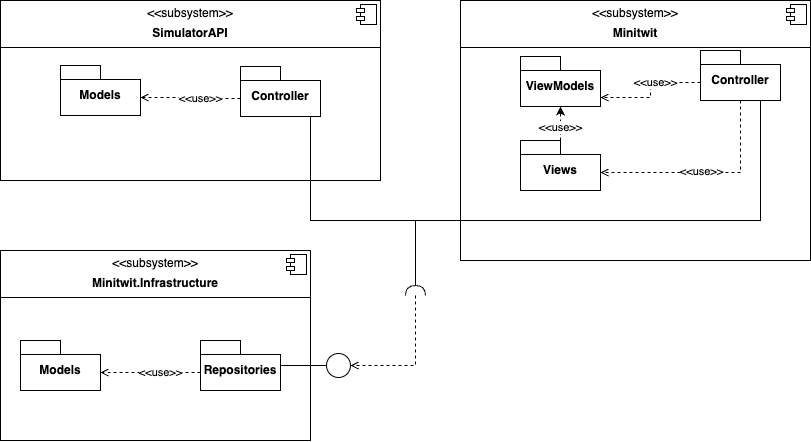
\includegraphics[width=1\textwidth]{Subsystem-Interaction.png}
    \end{center}
    \caption{An overview of subsystems and how they interact}
    \label{fig:subsystem-interaction}
\end{figure}

Although the two subsystems may look the same they handle request very differently. As can be seen in figure \ref{fig:frontend-interaction} the controller handles a lot of logic in order to present the correct information to the user. However, in figure \ref{fig:backend-interaction} there is little to non logic, and it only call the repository to fetch the user messages.
\begin{figure}[H]
    \begin{center}
        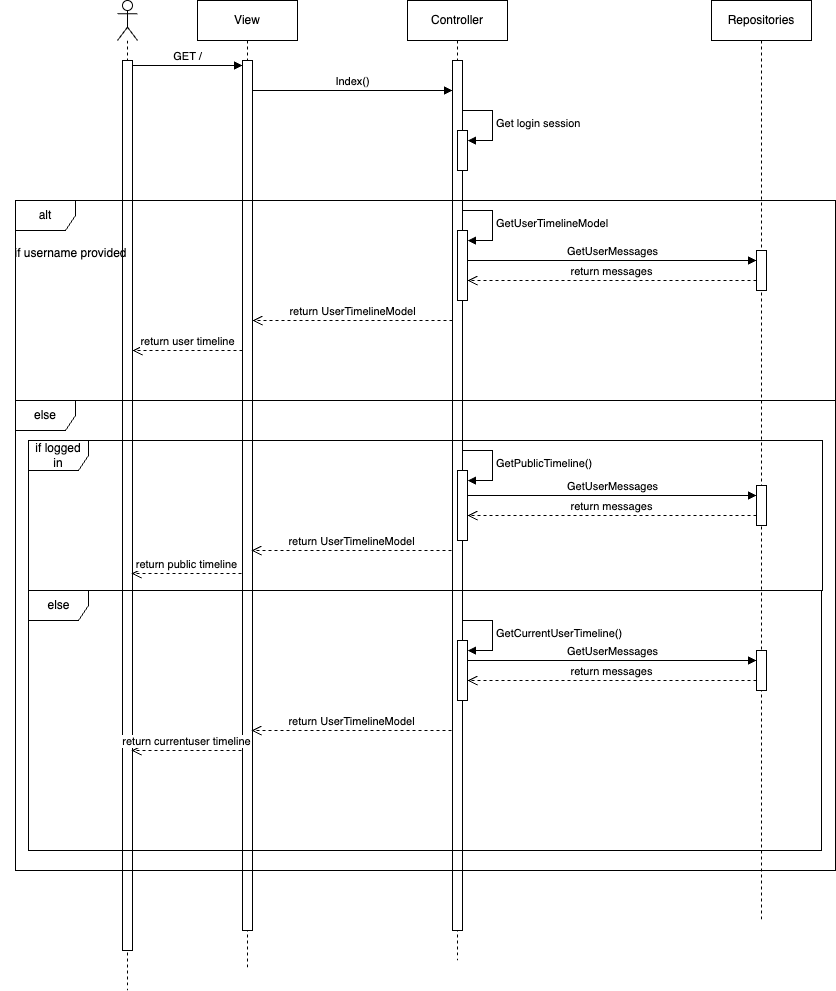
\includegraphics[width=1\textwidth]{Fronted-Sequence-Diagram.png}
    \end{center}
    \caption{Sequence diagram of a user call the index page}
    \label{fig:frontend-interaction}
\end{figure}
\begin{figure}[H]
    \begin{center}
        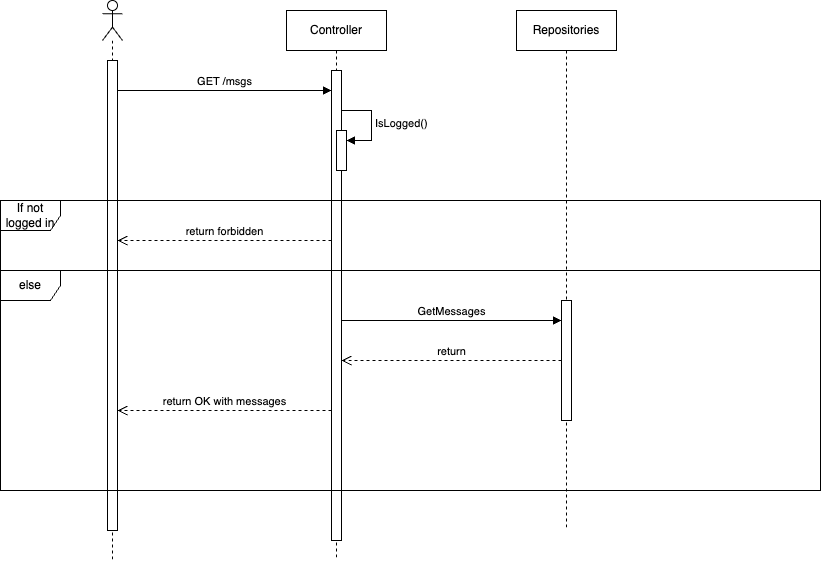
\includegraphics[width=1\textwidth]{Backend-Sequence-Diagram.png}
    \end{center}
    \caption{Sequence diagram of a user call the index page}
    \label{fig:backend-interaction}
\end{figure}
\subsubsection{Minitwit.Infrastructure}
In the previous section we saw that the controller logic is very different but needs to call the same queries.
Minitwit.Infrastructure is implemented to share duplicate code between the SimulatorAPI and Minitwit. This can be seen with the interaction of the package Repositories which leverages the Repository Pattern to abstract the logic of handling database queries and make it testable.


\subsection{Current state}
Table \ref{current-table} describes the status of the system after the simulator has been shut down.
\begin{table}[H]
    \begin{center}
        \begin{tabular}{ |c|c| }
            \hline
            Total requests & 34233 \\
            Requests secured & 34233 \\
            Total unhandled exceptions & 18 \\
            P99 min response time & 94.2 ms \\
            P99 max response time & 716 ms \\
            \hline
        \end{tabular}
    \end{center}
    \caption{System metrics}
    \label{current-table}
\end{table}
Furthermore, the static analysis tool Sonarcloud assesses that the quality of the overall code is good (see appendix \ref{appendix:sonarcloud}).
